\section{Method}
The method section first describes RECIST-guided regional cropping and prompt encoding, then introduces the MedNeXt-v2 segmentation model, and finally describes prompt-aware postprocessing and AutoZoom inference.


\subsection{Preprocessing}
\label{sec:input_preprocessing}

All CT volumes were resampled to a spacing of \(2.4 \times 1.0 \times 1.0\) mm in \(z,y,x\) order. For each RECIST annotation, we extracted a RECIST-centered regional crop of size \(72 \times 160 \times 160\) voxels. Predictions produced in crop space were mapped back to the original image grid after inference.

CT intensities were clipped to \([-999,255]\) HU and normalized by subtracting the training-set mean \(\mu=69.86\) and dividing by the training-set standard deviation \(\sigma=200.88\). The normalized crop is denoted by \(\tilde{\mathbf{I}}_{\mathrm{CT}}\).

LETT-NeXt conditions the segmentation model on RECIST annotations by concatenating two prompt channels with the normalized CT crop. The first channel, \(\mathbf{P}_{\mathrm{line}}\), is a binary RECIST-line mask. The two RECIST endpoints are connected on the axial RECIST slice and thickened with disks of radius \(r=2\) voxels. Voxels covered by the thickened line are assigned value 1, and all other voxels are assigned value 0.

The second channel, \(\mathbf{P}_{\mathrm{endpoints}}\), is an endpoint heatmap. For voxel coordinate \(\mathbf{v}=(z,y,x)\) and RECIST endpoints \(\mathbf{p}_1,\mathbf{p}_2\) in crop coordinates, the heatmap is defined as
\[
\mathbf{P}_{\mathrm{endpoints}}(\mathbf{v})
=
\max_{i \in \{1,2\}}
\exp
\left(
-\frac{
\left\| \mathbf{v} - \mathbf{p}_i \right\|_2^2
}{
2\sigma_{\mathrm{end}}^2
}
\right),
\]
where \(\sigma_{\mathrm{end}}=2.0\) voxels controls the spatial spread of the endpoint prompt.

The final network input is the three-channel tensor
\[
\mathbf{X}
=
\left[
\tilde{\mathbf{I}}_{\mathrm{CT}},
\mathbf{P}_{\mathrm{line}},
\mathbf{P}_{\mathrm{endpoints}}
\right].
\]

\subsection{Proposed Method}

Figure~\ref{fig:mednext_architecture} illustrates the LETT-NeXt segmentation network.
LETT-NeXt uses the three-channel input \(\mathbf{X}\) from Section~\ref{sec:input_preprocessing} and predicts a binary lesion mask with a compact MedNeXt-v2 f32 encoder--decoder~\cite{royMedNeXtv2Scaling3D2025}.
The network follows a 3D U-Net-like topology with skip connections between corresponding resolution levels and contains approximately 6.92 million trainable parameters.
Additional block-level details are provided in Appendix~\ref{app:mednext_blocks}.

\begin{figure}[t]
\centering
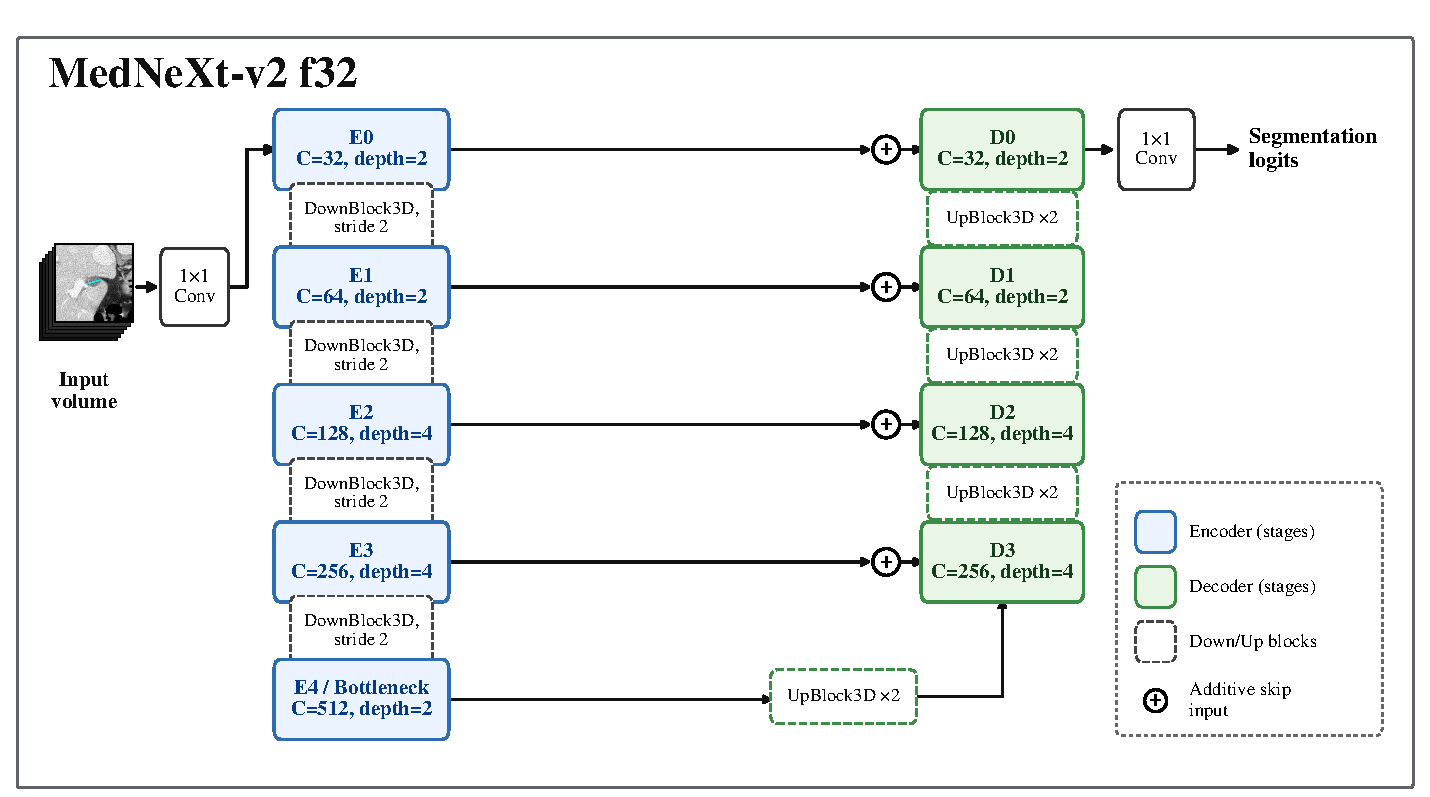
\includegraphics[width=\textwidth]{images/mednext_architecture.pdf}
\caption{
Overview of the MedNeXt-v2 f32 architecture used in LETT-NeXt.
The network has five encoder scales, four decoder scales, skip connections between corresponding resolution levels, and encoder channel widths of 32, 64, 128, 256, and 512.
}
\label{fig:mednext_architecture}
\end{figure}


\subsubsection{Auxiliary anatomy supervision}
\label{sec:auxiliary_anatomy_supervision}

During training, LETT-NeXt used a training-only auxiliary anatomy--tumor head in addition to the main RECIST-guided lesion segmentation head. This was motivated by anatomy-aware supervision in PanTS~\cite{liPanTSPancreaticTumor2025a}, and was used to encourage anatomy-aware feature learning around the prompted lesion.

The auxiliary head was implemented as a \(1 \times 1 \times 1\) convolution attached to the final decoder feature map. It predicted a local anatomy--tumor map for PanTS-supervised training crops, while the main RECIST-guided head predicted a binary lesion mask.

The auxiliary loss was computed only over voxels with valid PanTS-derived auxiliary labels. It combined multi-class cross-entropy and multi-class Dice loss over the auxiliary anatomy--tumor label space:
\[
\mathcal{L}_{\mathrm{aux}}
=
0.5\,\mathcal{L}_{\mathrm{CE}}
\left(
\hat{\mathbf{Y}}_{\mathrm{aux}},
\mathbf{Y}_{\mathrm{aux}}
\right)
+
0.5\,\mathcal{L}_{\mathrm{Dice}}^{\mathrm{multi}}
\left(
\hat{\mathbf{Y}}_{\mathrm{aux}},
\mathbf{Y}_{\mathrm{aux}}
\right).
\]
For crops without valid auxiliary labels, the auxiliary term was set to zero. At inference, only the main lesion head was used, and the auxiliary logits were ignored.


\subsection{Postprocessing}
\label{sec:inference_autozoom}
LETT-NeXt performed inference independently for each RECIST marker in a CT scan. 
Each prompt corresponds to one target lesion, so the pipeline produced one lesion prediction per RECIST marker. 
For each prompt, the corresponding input tensor \(\mathbf{X}\) was passed through the MedNeXt-v2 f32 model.
The sigmoid output was thresholded at 0.35 to obtain candidate lesion voxels. This value was selected by a validation-set threshold sweep.

To ensure that each prediction corresponded to a single prompted lesion, connected components were computed on the thresholded crop-space mask. 
The component most consistent with the RECIST marker was retained. 
Selection first used the component with the largest overlap with the RECIST marker region. 
If no component overlapped the prompt region, the component closest to the prompt center was selected instead. 
The selected crop-space mask was mapped back to the original image grid and assigned the corresponding RECIST label ID in the final output mask.

\subsubsection{AutoZoom}

AutoZoom is designed for cases where the initial RECIST-centered crop may not fully contain the lesion. Small crops preserve more image detail, but lesions that extend beyond the crop boundary can be truncated. Following the prompt-guided local inference strategy of nnInteractive~\cite{isenseeNnInteractiveRedefining3D2025}, LETT-NeXt performs a second inference pass only when the first-pass prediction touches the crop boundary.

For the second pass, a larger physical crop is extracted around the same RECIST marker, resized to the fixed network input size, and passed through the same model. The expanded prediction replaces the initial prediction, after which the same thresholding, component selection, and mapping procedure is applied.
